\documentclass{article}
\usepackage{geometry,amsmath,amssymb,theorem,caption,extarrows,mathrsfs,physics,bm}
\usepackage{graphicx,xcolor,listings,geometry,booktabs,subfigure,tikz}
\usepackage{pgfplots,grffile}
\pgfplotsset{compat=newest}
  %% the following commands are needed for some matlab2tikz features
\usetikzlibrary{plotmarks}
\usetikzlibrary{arrows.meta}
\usetikzlibrary{calc}
\usepgfplotslibrary{patchplots}
\usepackage{xeCJK,fontspec}
\setCJKmainfont[BoldFont=LXGW WenKai Bold]{LXGW WenKai Mono}
  \setCJKsansfont{黑体}%serif是有衬线字体sans serif无衬线字体。
  %\setmonofont{CMU Typewriter Text} % 等寬字型
  \XeTeXlinebreaklocale "zh"
  \XeTeXlinebreakskip = 0pt plus 1pt minus 0.1pt
\lstset{
    basicstyle          =   \sffamily,          % 基本代码风格
    keywordstyle        =   \bfseries,          % 关键字风格
    commentstyle        =   \rmfamily\itshape,  % 注释的风格,斜体
    stringstyle         =   \ttfamily,  % 字符串风格
    flexiblecolumns,                % 别问为什么,加上这个
    numbers             =   left,   % 行号的位置在左边
    showspaces          =   false,  % 是否显示空格,显示了有点乱,所以不现实了
    numberstyle         =   \zihao{-5}\ttfamily,    % 行号的样式,小五号,tt等宽字体
    showstringspaces    =   false,
    captionpos          =   t,      % 这段代码的名字所呈现的位置,t指的是top上面
    frame               =   tb,   % 显示边框
}

\lstdefinestyle{Python}{
    language        =   Python, % 语言选Python
    basicstyle      =   \zihao{-5}\ttfamily,
    numberstyle     =   \zihao{-5}\ttfamily,
    keywordstyle    =   \color{blue},
    keywordstyle    =   [2] \color{teal},
    stringstyle     =   \color{magenta},
    commentstyle    =   \color[HTML]{338AAF}\ttfamily,
    breaklines      =   true,   % 自动换行,建议不要写太长的行
    columns         =   fixed,  % 如果不加这一句,字间距就不固定,很丑,必须加
    basewidth       =   0.5em,
}
\definecolor{codegreen}{rgb}{0,0.6,0}
\definecolor{codegray}{rgb}{0.5,0.5,0.5}
\definecolor{codepurple}{rgb}{0.58,0,0.82}
\definecolor{backcolour}{rgb}{0.95,0.95,0.92}
\definecolor{hlinkblue}{rgb}{0.27,0.52,0.76}
\lstdefinestyle{mathematica}{
    backgroundcolor=\color{backcolour},
    commentstyle=\color[HTML]{338AAF}\ttfamily,
    keywordstyle=\zihao{-5}\sffamily\bfseries\color{magenta},
    numberstyle=\tiny\color{codegray},
    stringstyle=\color{codepurple},
    basicstyle=\zihao{-5}\ttfamily,
    breakatwhitespace=false,
    breaklines=true,
    basewidth=0.5em,
    captionpos=b,
    columns=fixed,
    keepspaces=true,
    numbers=left,
    numbersep=5pt,
    showspaces=false,
    showstringspaces=false,
    showtabs=false,
    tabsize=4
}
\lstdefinestyle{matlab}{
    language=matlab,
    backgroundcolor=\color{backcolour},
    commentstyle=\color[HTML]{338AAF}\ttfamily,
    keywordstyle=\zihao{-5}\sffamily\bfseries\color{magenta},
    numberstyle=\tiny\color{codegray},
    stringstyle=\color{codepurple},
    basicstyle=\zihao{-5}\ttfamily,
    breakatwhitespace=false,
    breaklines=true,
    basewidth=0.5em,
    captionpos=b,
    columns=fixed,
    keepspaces=true,
    numbers=left,
    numbersep=5pt,
    showspaces=false,
    showstringspaces=false,
    showtabs=false,
    tabsize=4
}
\newcommand{\dif}{\mathop{}\!\mathrm{d}}
\newcommand{\const}{\mathop{}\!\mathrm{const.}}
\newcommand{\splitline}{\noindent\rule[0.25\baselineskip]{\textwidth}{0.5pt}}
\newcommand{\autographinsert}[2]{\includegraphics[
  height=\dimexpr\pagegoal-\pagetotal-4\baselineskip\relax,width=#1\textwidth,
  keepaspectratio]{#2}}
  % NOTE: 插入图片如果出问题飘到下一页,请调整减掉的行数
\newtheorem{theorem}{定理}
\geometry{a4paper,left=1.8cm,right=1.8cm,top=1.5cm,bottom=1.5cm}
\begin{document}
    \title{Homework 2}
    \author{仇琨元 {\color{hlinkblue} \underline{11913019@mail.sustech.edu.cn}}}
    \date{\today}
    \maketitle

\section{Problem 2.2}
\subsection{No.3}

\begin{equation}
    \begin{aligned}
        y'&=\cos^{2}(x)\cos^{2}(2y)\\
        \Rightarrow \frac{\dif y}{\cos^{2}(2y)}&=\cos^{2}x \dif x\\
        \text{LHS:}\ \int_{}^{} \frac{\dif y}{\cos^{2}(2y)}&=\frac{\tan 2y}{2}+C_{1}\\
        \text{RHS:}\ \int_{}^{} \cos^{2}x \dif x&=\frac{x}{2}+\frac{\sin 2x}{4}+C_{2}\\
        y=\pm\frac{1}{2} \tan^{-1}\left( \pm \left( x+\frac{\sin 2x}{2}+C \right)  \right)
    \end{aligned}
\end{equation}

\subsection{No.5}
\begin{equation}
    \begin{aligned}
        y'&=\frac{x-e^{-x}}{y+e^{y}}\\
        (y+e^{y})\dif y&=(x-e^{-x})\dif x\\
        \frac{y^{2}}{2}+e^{y}&=\frac{x^{2}}{2}+e^{-x}+C
    \end{aligned}
\end{equation}

Since the LHS of eq(2) is transcendent, the further simplification is not possible.

\subsection{No.9}

(a)

General solution:

\begin{equation}
    \begin{aligned}
        y^{-2}\dif y&=(1-2x)\dif x\\
        -y^{-1}&=x-x^{2}+C_{1}\\
        y=\frac{1}{x(x-1)+C_{2}}
    \end{aligned}
\end{equation}

Specific solution:
\begin{equation}
    \begin{aligned}
        y(0)&=\frac{1}{C_{2}}=-\frac{1}{6}\\
        C_{2}&=-6\\
        y_{p}&=\frac{1}{x^2-x-6}\\
        &=\frac{1}{(x+2)(x-3)}
    \end{aligned}
\end{equation}

(b)

Plot:
\begin{figure}
    \begin{small}
        \begin{center}
            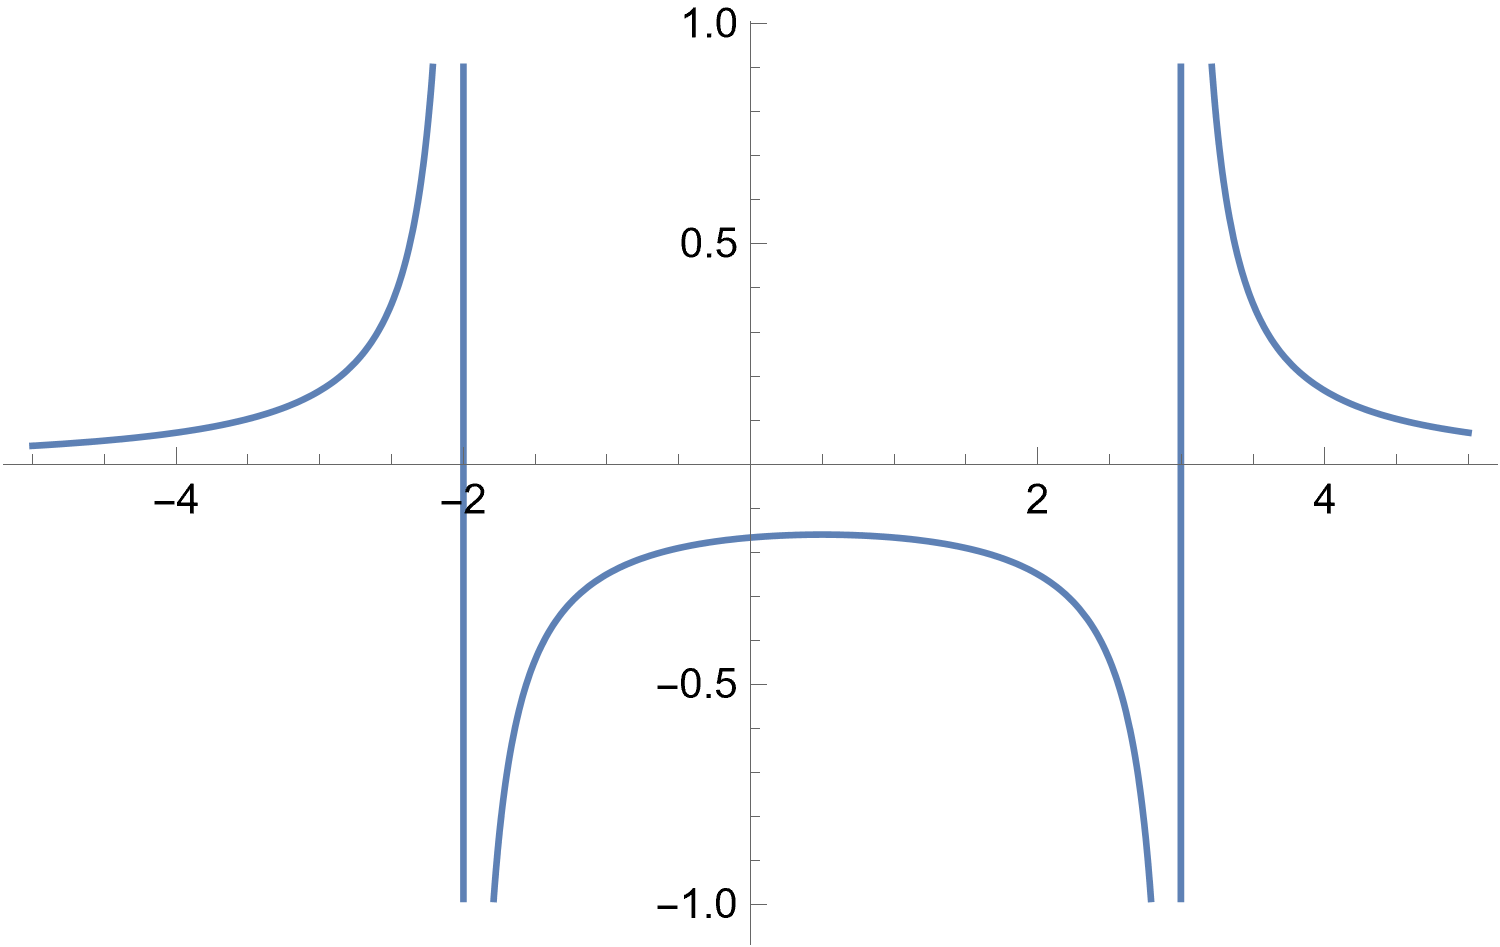
\includegraphics[width=0.95\textwidth]{figures/prob229.png}
        \end{center}
        \caption{Specific Solution at \( y(0)=-1/6 \) }
        \label{fig:sol_spec_229}
    \end{small}
\end{figure}


\end{document}